\section{Estimation of the $\tau\tau$ mass}

The final signal extraction is done to the total $\tau\tau$ mass, which is estimated from the visible $\tau\tau$ mass using the FastMTT algorithm \cite{2014_SVFit_Bianchini}. FastMTT is based on the SVFit algorithm, originally developed for the Standard Model $H \rightarrow \tau\tau$ analysis \cite{CMS-HIG-13-004}. Both the SVFit algorithms, and the FastMTT algorithm, are described below, to give a complete picture of how tau decays are parametrized.

To specify a hadronic $\tau$ decay, six parameters are needed \cite{CMS-HIG-13-004}: the polar and azimuthal angles of the visible decay product system in the $\tau$ rest frame, the three boost parameters from the $\tau$ rest frame to the laboratory frame, and the invariant mass $m_{\text{vis}}$ of the visible decay products. For a leptonic $\tau$ decay, two neutrinos are produced, and a seventh parameter, the invariant mass of the two-neutrino system, is necessary. The unknown parameters are constrained by four observables that are the components of the four-momentum of the system formed by the visible decay products of the $\tau$ lepton, measured in the laboratory frame. The remaining unconstrained parameters for hadronic and leptonic $\tau$ decays are thus:

\begin{itemize}
    \item The fraction of the $\tau$ energy in the laboratory frame carried by the visible decay products,
    \item $\phi$, the azimuthal angle of the $\tau$ direction in the laboratory frame,
    \item $m_\nu\nu$, the invariant mass of the two-neutrino system in leptonic $\tau$ decays (for hadronic $\tau$ decays, $m_{\nu\nu}$ is set to 0).
\end{itemize}
$E_{x}^{\text{miss}}$ and $E_{y}^{\text{miss}}$, the $x$ and $y$ components of the missing transverse energy $E_{T}^{\text{miss}}$ provide two further constraints. 

\subsection{Original SVFit ``standalone'': maximum likelihood}
In one of the original versions of SVFit, called ``standalone'' SVFit \cite{CMS-HIG-13-004}, a maximum likelihood fit method is used to reconstruct the mass $m_{\tau\tau}$ by combining the measured observables $E_{x}^{\text{miss}}$ and $E_{y}^{\text{miss}}$ with a likelihood model that includes terms for the $\tau$ decay kinematics and the $E_{T}^{\text{miss}}$ resolution \cite{CMS-HIG-13-004}. The likelihood function $f(\vec{z}, \vec{y}, \vec{a}_1 \vec{a}_2)$ of the parameters $\vec{z} = (E_{x}^{\text{miss}}, E_{y}^{\text{miss}})$ in an event is constructed, where the remaining parameters are the kinematics of the two $\tau$ decays, denoted $\vec{a}_1 = (x_1, \phi_1, m_{\nu\nu, 1})$ and $\vec{a}_2 = (x_2, \phi_2, m_{\nu\nu, 2})$, and the four-momenta of the visible decay products with the measured values $\vec{y} = (p_1^{\text{vis}}, p_2^{\text{vis}})$.

The likelihood $f$ is the product of three likelihood functions. The first two likelihood functions model the decay parameters $\vec{a}_1$ and $\vec{a}_2$ of the two $\tau$ leptons. For leptonic decays, the likelihood function is modeled using matrix elements for $\tau$ decays, and integrated over the allowed phase space $0 \leq x \leq 1$ and $0 \leq m_{\nu\nu} \leq m_{\tau} \sqrt{1-x}$. For hadronic $\tau$ decays, a model based on the two-body phase space is used and integrated over $m_{\text{vis}}^2/ m_{\tau\tau}^2 \leq x \leq 1$. The third likelihood function quantifies the compatibility of a $\tau$ decay hypothesis with the reconstructed $\vec{E}_{T}^{\text{miss}}$ in an event, assuming the neutrinos are the only source of missing transverse energy. The expected $\vec{E}_{T}^{\text{miss}}$ resolution is represented by a covariant matrix, estimated on an event-by-event basis using a significance algorithm \cite{CMS-JME-10-009}.

\subsection{``Classic SVFit" with matrix element}
Classic SVFit is an improved algorithm of the original ``standalone" SVFit using the formalism of the matrix element (ME) method \cite{2014_SVFit_Bianchini}. In the ME method, an estimate for the unknown model parameter $\Theta$ (here, the mass $m_{\tau\tau}$) is obtained by maximizing the probability density $\mathcal{P}$. The key ingredients of the probability density are the squared modulus of the matrix element $|\mathcal{M}(\mathbf{p}, \Theta)|^2$ and the transfer function $W(\mathbf{y}|\mathbf{p})$ (probability density to observe the measured observables $\mathbf{y}$ given the phase space point $\mathbf{p}$). The best estimate $m_{\tau\tau}$ is obtained by computing the probability density $\mathcal{P}$ for a range of mass hypotheses and finding the value of $m_{\tau\tau}$ that maximizes $\mathcal{P}$.

Distributions illustrating the performance of the classic matrix element SVFit algorithm are shown in Fig. \ref{fig:classic_svfit_resolution} from \cite{2014_SVFit_Bianchini}, showing the di-tau mass after and before application of SVFit to recover energy lost to neutrinos. The SVFit algorithm is found to improve the sensitivity of the Standard Model $H \rightarrow \tau\tau$ analysis performed by CMS by about 30\%, compared to performing the same analysis using only the visible mass $m_{\text{vis}}$. 

\begin{figure}[ht]
    \centering
    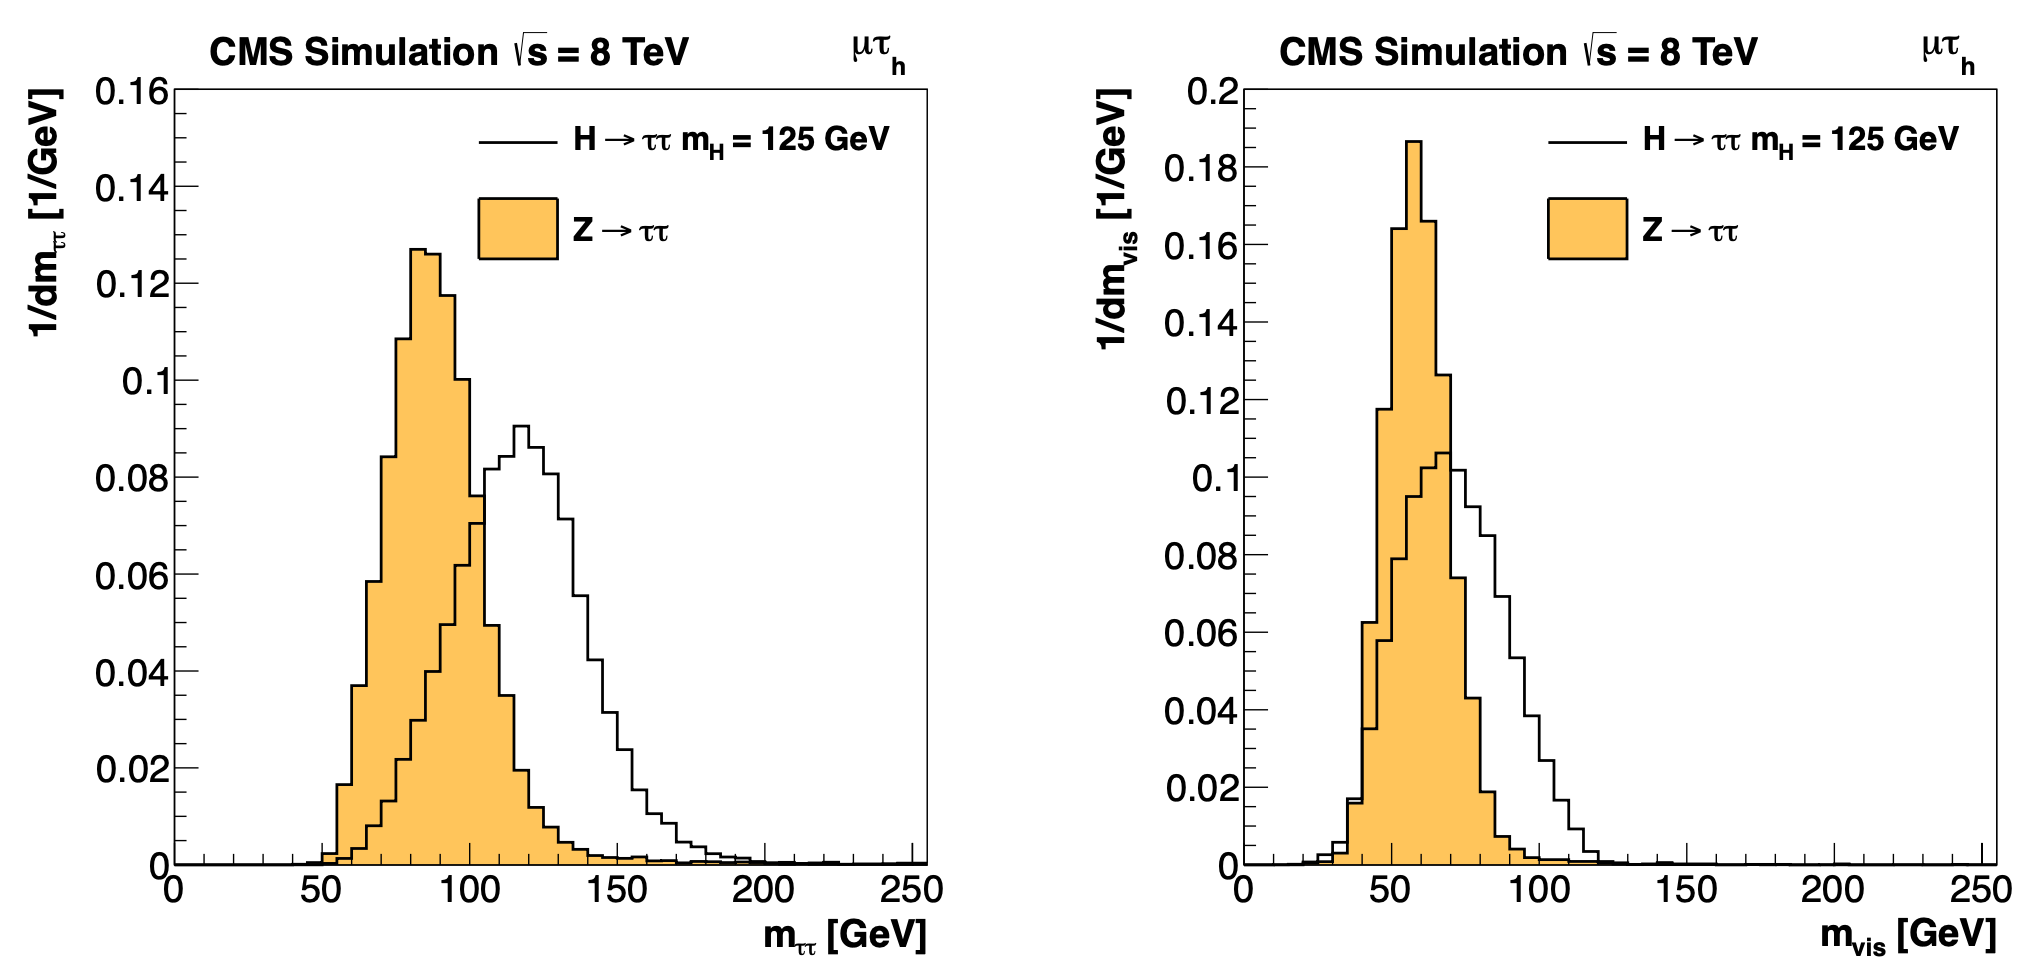
\includegraphics[width=15cm]{figures/ch-12-signal-extraction-statistical-fitting/original_SVFit_resolution_2014_SVFit_Bianchini.png}
    \caption[Distributions of $m_{\tau\tau}$ reconstructed by the classic SVFit algorithm, and masses of visible tau decay products (before SVFit).]{Distributions from \cite{2014_SVFit_Bianchini}, of $m_{\tau\tau}$ after reconstruction with the original SVFit algorithm (\textit{left}), and before SVFit with only the visible tau decay products (\textit{right}), for $H \rightarrow \tau\tau$ signal events of mass $m_H = 125$ GeV (\textit{black line}) and the $Z/\gamma^* \rightarrow \tau\tau$ background (\textit{orange, solid}), in the decay channel $\tau\tau \rightarrow \mu\tau_{h}$.} 
    \label{fig:classic_svfit_resolution}
\end{figure}


\subsection{FastMTT: optimized SVFit}
FastMTT \cite{CMS-AN-19-032-FastMTT} is a further simplification to the matrix element method of Classic SVFit which has comparable performance but is about 100 times faster. FastMTT drops the matrix element component of the computation without significant impact on the final mass resolution, and simplifies the computation of the transfer functions. The opening angle of the $\tau$ decay products with respect to the initial $\tau$ momenta approaches 0 for $\tau$ with high $\gamma = E_{\tau}/m_{\tau}$, with typical $\tau$ decays from the Z boson decays already satisfying this condition. In this collinear approximation, the dimensionality of the transfer function can be reduced in the computation of FastMTT, while still yielding similar results to Classic SVFit \cite{CMS-AN-19-032-FastMTT}. 


\section{Signal extraction}

A binned maximum likelihood fit is performed on the $m_{\tau\tau}$ distribution with the systematic uncertainties described in Chapter \ref{chapter:ch-11:systematic-uncertainties}. Event categories described in Section \ref{chapter:ch-10:event-categorization}, in all three channels, are included in a simultaneous fit. 

Limits and confidence intervals are obtained using the modified frequentist CL$_s$ approach, with an asymptotic approximation to the distribution of the profile likelihood test statistic.

